
%Preámbulo:
\documentclass[12pt,a4paper]{article}

\usepackage{graphicx}
\usepackage{bm}
\usepackage[utf8]{inputenc}
% caracteres utf8 (tildes, enie) sin tener que usar comandos

\usepackage{pdfpages} 
%para agregar pdfs(Karnaugh)

\usepackage[spanish, es-tabla, es-nodecimaldot]{babel}
% texto automatico en espaniol
% "tabla" en vez de "cuadro"
% no reemplaza puntos decimales por comas

%%%%%%%%%%%%%%%%%%%%%%%%%%%%%%%%%
%%%%%%%% PAQUETES EXTRA %%%%%%%%%
%%%%%%%%%%%%%%%%%%%%%%%%%%%%%%%%%

%Defino el papel y caracteristicas del informe
\usepackage[a4paper, total={6in, 8in}]{geometry}
\setlength{\parindent}{10pt}			%cuanta sangria al principio de un parrafo
\usepackage{indentfirst}				%pone sangria al primer parrafo de una seccion
\usepackage{graphicx} % importar imagenes
\usepackage{float} % posicion H para floats
\usepackage[colorinlistoftodos]{todonotes}
%Para realizar los mapas de Karnaugh (Sacado de https://tex.stackexchange.com/questions/140567/drawing-karnaughs-maps-in-latex)
%Macro para tablas de Karnaugh 
\usepackage{tikz}
\usetikzlibrary{matrix,calc}

%isolated term
%#1 - Optional. Space between node and grouping line. Default=0
%#2 - node
%#3 - filling color
\newcommand{\implicantsol}[3][0]{
    \draw[rounded corners=3pt, fill=#3, opacity=0.3] ($(#2.north west)+(135:#1)$) rectangle ($(#2.south east)+(-45:#1)$);}

%internal group
%#1 - Optional. Space between node and grouping line. Default=0
%#2 - top left node
%#3 - bottom right node
%#4 - filling color
\newcommand{\implicant}[4][0]{
    \draw[rounded corners=3pt, fill=#4, opacity=0.3] ($(#2.north west)+(135:#1)$) rectangle ($(#3.south east)+(-45:#1)$);
    }

%group lateral borders
%#1 - Optional. Space between node and grouping line. Default=0
%#2 - top left node
%#3 - bottom right node
%#4 - filling color
\newcommand{\implicantcostats}[4][0]{
    \draw[rounded corners=3pt, fill=#4, opacity=0.3] ($(rf.east |- #2.north)+(90:#1)$)-| ($(#2.east)+(0:#1)$) |- ($(rf.east |- #3.south)+(-90:#1)$);
    \draw[rounded corners=3pt, fill=#4, opacity=0.3] ($(cf.west |- #2.north)+(90:#1)$) -| ($(#3.west)+(180:#1)$) |- ($(cf.west |- #3.south)+(-90:#1)$);
}

%group top-bottom borders
%#1 - Optional. Space between node and grouping line. Default=0
%#2 - top left node
%#3 - bottom right node
%#4 - filling color
\newcommand{\implicantdaltbaix}[4][0]{
    \draw[rounded corners=3pt, fill=#4, opacity=0.3] ($(cf.south -| #2.west)+(180:#1)$) |- ($(#2.south)+(-90:#1)$) -| ($(cf.south -| #3.east)+(0:#1)$);
    \draw[rounded corners=3pt, fill=#4, opacity=0.3] ($(rf.north -| #2.west)+(180:#1)$) |- ($(#3.north)+(90:#1)$) -| ($(rf.north -| #3.east)+(0:#1)$);
}

%group corners
%#1 - Optional. Space between node and grouping line. Default=0
%#2 - filling color
\newcommand{\implicantcantons}[2][0]{
    \draw[rounded corners=3pt, opacity=.3] ($(rf.east |- 0.south)+(-90:#1)$) -| ($(0.east |- cf.south)+(0:#1)$);
    \draw[rounded corners=3pt, opacity=.3] ($(rf.east |- 8.north)+(90:#1)$) -| ($(8.east |- rf.north)+(0:#1)$);
    \draw[rounded corners=3pt, opacity=.3] ($(cf.west |- 2.south)+(-90:#1)$) -| ($(2.west |- cf.south)+(180:#1)$);
    \draw[rounded corners=3pt, opacity=.3] ($(cf.west |- 10.north)+(90:#1)$) -| ($(10.west |- rf.north)+(180:#1)$);
    \fill[rounded corners=3pt, fill=#2, opacity=.3] ($(rf.east |- 0.south)+(-90:#1)$) -|  ($(0.east |- cf.south)+(0:#1)$) [sharp corners] ($(rf.east |- 0.south)+(-90:#1)$) |-  ($(0.east |- cf.south)+(0:#1)$) ;
    \fill[rounded corners=3pt, fill=#2, opacity=.3] ($(rf.east |- 8.north)+(90:#1)$) -| ($(8.east |- rf.north)+(0:#1)$) [sharp corners] ($(rf.east |- 8.north)+(90:#1)$) |- ($(8.east |- rf.north)+(0:#1)$) ;
    \fill[rounded corners=3pt, fill=#2, opacity=.3] ($(cf.west |- 2.south)+(-90:#1)$) -| ($(2.west |- cf.south)+(180:#1)$) [sharp corners]($(cf.west |- 2.south)+(-90:#1)$) |- ($(2.west |- cf.south)+(180:#1)$) ;
    \fill[rounded corners=3pt, fill=#2, opacity=.3] ($(cf.west |- 10.north)+(90:#1)$) -| ($(10.west |- rf.north)+(180:#1)$) [sharp corners] ($(cf.west |- 10.north)+(90:#1)$) |- ($(10.west |- rf.north)+(180:#1)$) ;
}

%Empty Karnaugh map 4x4
\newenvironment{Karnaugh}%
{
\begin{tikzpicture}[baseline=(current bounding box.north),scale=0.8]
\draw (0,0) grid (4,4);
\draw (0,4) -- node [pos=0.7,above right,anchor=south west] {$X_1X_2$} node [pos=0.7,below left,anchor=north east] {$X_3X_4$} ++(135:1);
%
\matrix (mapa) [matrix of nodes,
        column sep={0.8cm,between origins},
        row sep={0.8cm,between origins},
        every node/.style={minimum size=0.3mm},
        anchor=8.center,
        ampersand replacement=\&] at (0.5,0.5)
{
                       \& |(c00)| 00         \& |(c01)| 01         \& |(c11)| 11         \& |(c10)| 10         \& |(cf)| \phantom{00} \\
|(r00)| 00             \& |(0)|  \phantom{0} \& |(1)|  \phantom{0} \& |(3)|  \phantom{0} \& |(2)|  \phantom{0} \&                     \\
|(r01)| 01             \& |(4)|  \phantom{0} \& |(5)|  \phantom{0} \& |(7)|  \phantom{0} \& |(6)|  \phantom{0} \&                     \\
|(r11)| 11             \& |(12)| \phantom{0} \& |(13)| \phantom{0} \& |(15)| \phantom{0} \& |(14)| \phantom{0} \&                     \\
|(r10)| 10             \& |(8)|  \phantom{0} \& |(9)|  \phantom{0} \& |(11)| \phantom{0} \& |(10)| \phantom{0} \&                     \\
|(rf) | \phantom{00}   \&                    \&                    \&                    \&                    \&                     \\
};
}%
{
\end{tikzpicture}
}

%Empty Karnaugh map 2x4
\newenvironment{Karnaughvuit}%
{
\begin{tikzpicture}[baseline=(current bounding box.north),scale=0.8]
\draw (0,0) grid (4,2);
\draw (0,2) -- node [pos=0.7,above right,anchor=south west] {$X_1X_2$} node [pos=0.7,below left,anchor=north east] {$X_3$} ++(135:1);
%
\matrix (mapa) [matrix of nodes,
        column sep={0.8cm,between origins},
        row sep={0.8cm,between origins},
        every node/.style={minimum size=0.3mm},
        anchor=4.center,
        ampersand replacement=\&] at (0.5,0.5)
{
                      \& |(c00)| 00         \& |(c01)| 01         \& |(c11)| 11         \& |(c10)| 10         \& |(cf)| \phantom{00} \\
|(r00)| 0             \& |(0)|  \phantom{0} \& |(1)|  \phantom{0} \& |(3)|  \phantom{0} \& |(2)|  \phantom{0} \&                     \\
|(r01)| 1             \& |(4)|  \phantom{0} \& |(5)|  \phantom{0} \& |(7)|  \phantom{0} \& |(6)|  \phantom{0} \&                     \\
|(rf) | \phantom{00}  \&                    \&                    \&                    \&                    \&                     \\
};
}%
{
\end{tikzpicture}
}

%Empty Karnaugh map 2x2
\newenvironment{Karnaughquatre}%
{
\begin{tikzpicture}[baseline=(current bounding box.north),scale=0.8]
\draw (0,0) grid (2,2);
\draw (0,2) -- node [pos=0.7,above right,anchor=south west] {$X_1$} node [pos=0.7,below left,anchor=north east] {$X_2$} ++(135:1);
%
\matrix (mapa) [matrix of nodes,
        column sep={0.8cm,between origins},
        row sep={0.8cm,between origins},
        every node/.style={minimum size=0.3mm},
        anchor=2.center,
        ampersand replacement=\&] at (0.5,0.5)
{
          \& |(c00)| 0          \& |(c01)| 1  \\
|(r00)| 0 \& |(0)|  \phantom{0} \& |(1)|  \phantom{0} \\
|(r01)| 1 \& |(2)|  \phantom{0} \& |(3)|  \phantom{0} \\
};
}%
{
\end{tikzpicture}
}

%Defines 8 or 16 values (0,1,X)
\newcommand{\contingut}[1]{%
\foreach \x [count=\xi from 0]  in {#1}
     \path (\xi) node {\x};
}

%Places 1 in listed positions
\newcommand{\minterms}[1]{%
    \foreach \x in {#1}
        \path (\x) node {1};
}

%Places 0 in listed positions
\newcommand{\maxterms}[1]{%
    \foreach \x in {#1}
        \path (\x) node {0};
}

%Places X in listed positions
\newcommand{\indeterminats}[1]{%
    \foreach \x in {#1}
        \path (\x) node {X};
}


\begin{document}

\newgeometry{} %Margenes default para la caratula
%Caratula:

\begin{titlepage}
    \newcommand{\HRule}{\rule{\linewidth}{0.5mm}}
    \begin{center}
    \mbox{\textsc{\large \bfseries {INSTITUTO TECNOL\'OGICO DE BUENOS AIRES}}}\\[1cm]
    \textsc{\Large 22.12 - Electr\'onica III}\\[0.5cm]
    
    \HRule \\[0.6cm]
    { \Huge \bfseries Trabajo Pr\'actico \bm{$N^\circ1$}}\\[0.4cm] 
    \HRule \\[1.5cm]
    
    
    \large
    
    \emph{\Large Grupo 4}\\
    \vspace{10px}
    
    \begin{tabular}{lr}
    \textsc{Bertachini}, Germ\'an  & 58750 \\ 	
    \textsc{Dieguez}, Manuel  & 56273 \\
    \textsc{Galdeman}, Agust\'in  & 59827 \\
    \textsc{Laguingue}, Juan Mart\'in  & 57430 \\
    \end{tabular} \\
    \vspace{20px}
    \begin{tabular}{lr}
    \textsc{}Profesores:\\
    \textsc{Dewald}, Kevin\\
    \textsc{Wundes}, Pablo\\
    \end{tabular}
    \vspace{60px}


    
\includegraphics[scale=0.20]{Extras/ITBA.png}    

    
    
    \vspace{30px}
    
    \textsc{\large Presentado el 5 de Septiembre de 2019}\\
    
    \end{center}
    
    \end{titlepage}


%Indice:
\tableofcontents
\newpage

% cambio los margenes para el resto del documento
\newgeometry{total={7in, 9in}}
%Ejercicios:
\section{Ejercicio 3 - Implementación de módulos en verilog}
A continuación, se implementarán los circuitos pedidos en lenguaje verilog, comentando como fue su desarrollo e emplementación.
\subsection{DEMUX de 4 salidas}

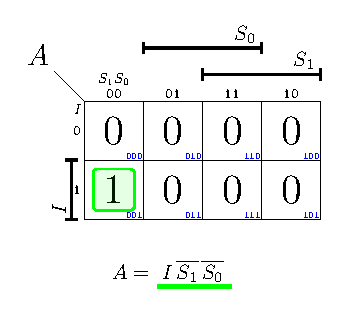
\includepdf{Ejercicio_3/Karnaugh/DEMUX/Salida_A.pdf}
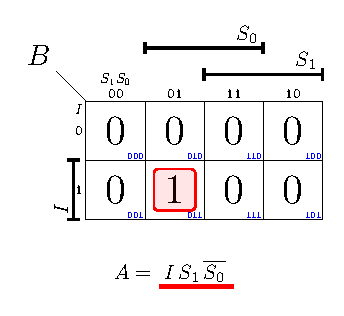
\includepdf{Ejercicio_3/Karnaugh/DEMUX/Salida_B.pdf}
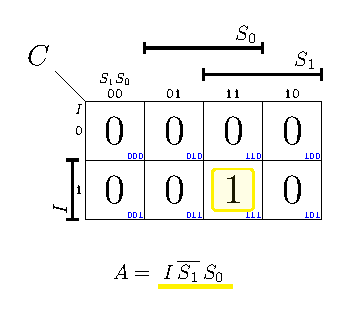
\includepdf{Ejercicio_3/Karnaugh/DEMUX/Salida_C.pdf}
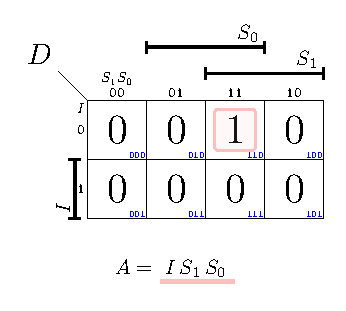
\includepdf{Ejercicio_3/Karnaugh/DEMUX/Salida_D.pdf}

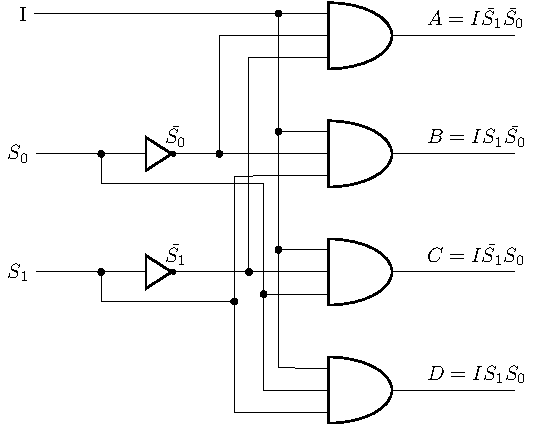
\includepdf{Ejercicio_3/Circuitos/Circuito_DEMUX.pdf}

\begin{table}[H]
	\begin{center}
		\begin{tabular}{ccc||cccc}

			$D$ &	$C_1$ &	$C_0$ &	$O_3$ & $O_2$ & $O_1$ &$O_0$ \\
			\hline
            0 & 0 & 0 & 0 & 0 & 0 & 0 \\
            
            0 & 0 & 1 & 0 & 0 & 0 & 0 \\
            
            0 & 1 & 0 & 0 & 0 & 0 & 0 \\
            
            0 & 1 & 1 & 0 & 0 & 0 & 0 \\
            
            1 & 0 & 0 & 1 & 0 & 0 & 0 \\
            
            1 & 0 & 1 & 0 & 1 & 0 & 0 \\
            
            1 & 1 & 0 & 0 & 0 & 1 & 0 \\
            
            1 & 1 & 1 & 0 & 0 & 0 & 1\\
			
		\end{tabular}
	\end{center}
\end{table}

\subsection{ENCODER de 4 entradas}

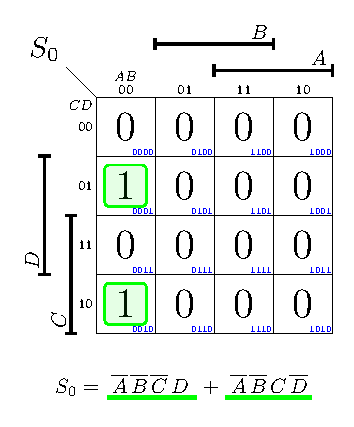
\includepdf{Ejercicio_3/Karnaugh/ENCODER/Salida_S_0.pdf}
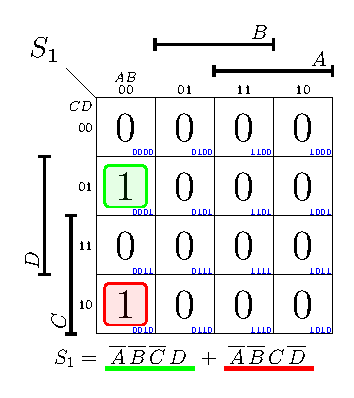
\includepdf{Ejercicio_3/Karnaugh/ENCODER/Salida_S_1.pdf}

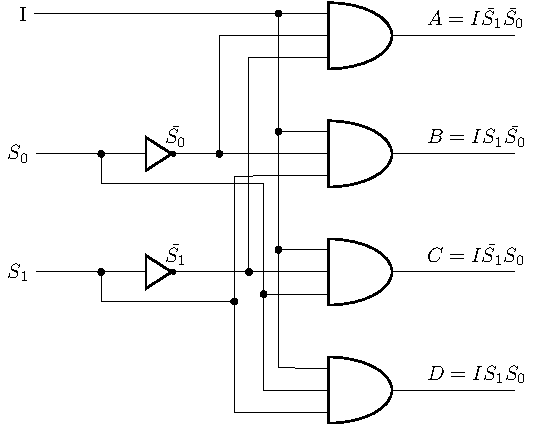
\includepdf{Ejercicio_3/Circuitos/Circuito_DEMUX.pdf}

\begin{table}[H]
	\begin{center}
		\begin{tabular}{c c c c||c c}

			$D$ &	$C$ &	$B$ &	$A$ & $S_1$ & $S_0$ \\
			\hline
            0 & 0 & 0 & 0 & 0 & 0   \\

            0 & 0 & 0 & 1 & 0 & 0   \\
  
            0 & 0 & 1 & 0 & 0 & 1   \\
          
            0 & 0 & 1 & 1 & 0 & 0   \\
         
            0 & 1 & 0 & 0 & 1 & 0   \\
           
            0 & 1 & 0 & 1 & 0 & 0   \\
         
            0 & 1 & 1 & 0 & 0 & 0   \\
        
            0 & 1 & 1 & 1 & 0 & 0   \\
         
            1 & 0 & 0 & 0 & 1 & 1   \\
        
            1 & 0 & 0 & 1 & 0 & 0   \\
         
            1 & 0 & 1 & 0 & 0 & 0   \\
       
            1 & 0 & 1 & 1 & 0 & 0  \\
          
            1 & 1 & 0 & 0 & 0 & 0   \\
      
            1 & 1 & 0 & 1 & 0 & 0   \\
        
            1 & 1 & 1 & 0 & 0 & 0   \\
          
            1 & 1 & 1 & 1 & 0 & 0  \\
		
		\end{tabular}
	\end{center}
\end{table}
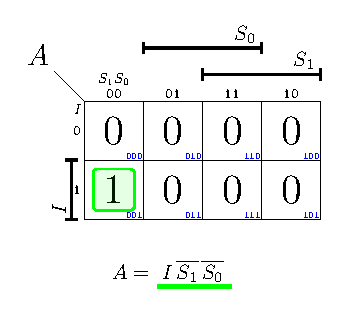
\includepdf[page={1}]{Ejercicio_3/Karnaugh/DEMUX/Salida_A.pdf}
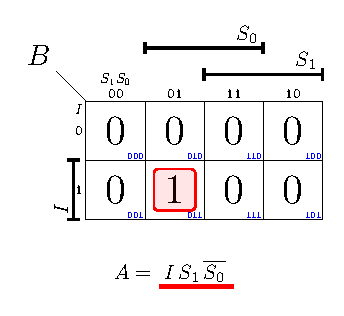
\includepdf[page={1}]{Ejercicio_3/Karnaugh/DEMUX/Salida_B.pdf}
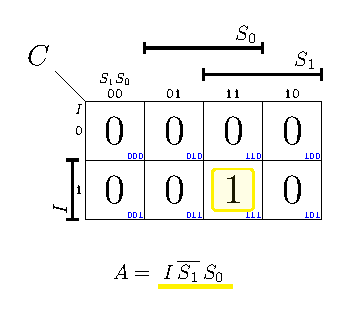
\includepdf[page={1}]{Ejercicio_3/Karnaugh/DEMUX/Salida_C.pdf}
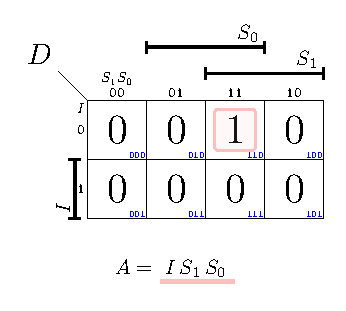
\includepdf[page={1}]{Ejercicio_3/Karnaugh/DEMUX/Salida_D.pdf}
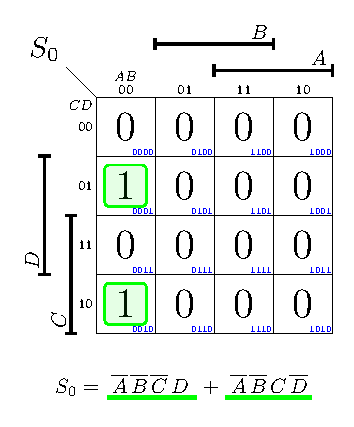
\includepdf[page={1}]{Ejercicio_3/Karnaugh/ENCODER/Salida_S_0.pdf}
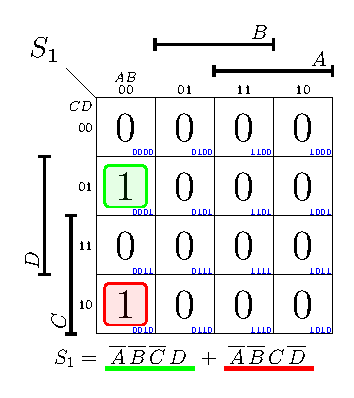
\includepdf[page={1}]{Ejercicio_3/Karnaugh/ENCODER/Salida_S_1.pdf}
\section{Conversor a codigo de Gray}
Para esté ejercicio, realizamos el desarrollo de un circuito lógico capaz de convertir un número binario de 4 bits a su equivalente de código de Gray, esto resulta en la siguiente tabla de verdad:
\begin{table}[H]
	\begin{center}
		\begin{tabular}{|c|c|c|c||c|c|c|c|}
			\hline
			\multicolumn{4}{|c||}{Entrada} & \multicolumn{4}{|c|}{Salida}\\
			\hline
			$X_1$ &	$X_2$ &	$X_3$ &	$X_4$ & $Y_1$ & $Y_2$ & $Y_3$ & $Y_4$\\
			\hline
			0 & 0 & 0 & 0 & 0 & 0 & 0 & 0\\
			\hline
			0 & 0 & 0 & 1 & 0 & 0 & 0 & 1\\
			\hline
			0 & 0 & 1 & 0 & 0 & 0 & 1 & 1\\
			\hline
			0 & 0 & 1 & 1 & 0 & 0 & 1 & 0\\
			\hline
			0 & 1 & 0 & 0 & 0 & 1 & 1 & 0\\
			\hline
			0 & 1 & 0 & 1 & 0 & 1 & 1 & 1\\
			\hline
			0 & 1 & 1 & 0 & 0 & 1 & 0 & 1\\
			\hline
			0 & 1 & 1 & 1 & 0 & 1 & 0 & 0\\
			\hline
			1 & 0 & 0 & 0 & 1 & 1 & 0 & 0\\
			\hline
			1 & 0 & 0 & 1 & 1 & 1 & 0 & 1\\
			\hline
			1 & 0 & 1 & 0 & 1 & 1 & 1 & 1\\
			\hline
			1 & 0 & 1 & 1 & 1 & 1 & 1 & 0\\
			\hline
			1 & 1 & 0 & 0 & 1 & 0 & 1 & 0\\
			\hline
			1 & 1 & 0 & 1 & 1 & 0 & 1 & 1\\
			\hline
			1 & 1 & 1 & 0 & 1 & 0 & 0 & 1\\
			\hline
			1 & 1 & 1 & 1 & 1 & 0 & 0 & 0\\
			\hline
		\end{tabular}
	\end{center}
\end{table}
De la tabla de verdad obtenemos las siguientes ecuaciones en función de los mintérminos:
\begin{center}
	$Y_4=m_1+m_2+m_5+m_6+m_9+m_{10}+m_{13}+m_{14}$\\
	$Y_3=m_2+m_3+m_4+m_5+m_{10}+m_{11}+m_{12}+m_{13}$\\
	$Y_2=m_4+m_5+m_6+m_7+m_8+m_9+m_{10}+m_{11}$\\
	$Y_1=m_8+m_9+m_{10}+m_{11}+m_{12}+m_{13}+m_{14}+m_{15}$\\
\end{center}
Que al reemplazar cada mintérmino por su correspondiente expresión obtenemos:
\begin{center}
	$Y_4=\overline{X_1} \cdot \overline{X_2} \cdot \overline{X_3} \cdot X_4 + 
	\overline{X_1} \cdot \overline{X_2} \cdot X_3 \cdot \overline{X_4} + 
	\overline{X_1} \cdot X_2 \cdot \overline{X_3} \cdot X_4 + 
	\overline{X_1} \cdot X_2 \cdot X_3 \cdot \overline{X_4} + 
	X_1 \cdot \overline{X_2} \cdot \overline{X_3} \cdot X_4 +
	X_1 \cdot \overline{X_2} \cdot X_3 \cdot \overline{X_4} + 
	X_1 \cdot X_2 \cdot \overline{X_3} \cdot X_4 + 
	X_1 \cdot X_2 \cdot X_3 \cdot \overline{X_4}$\\
	\smallskip
	%Empieza la parte Y3%
	$Y_3=\overline{X_1} \cdot \overline{X_2} \cdot X_3 \cdot \overline{X_4} +
	\overline{X_1} \cdot \overline{X_2} \cdot X_3 \cdot X_4 +
	\overline{X_1} \cdot X_2 \cdot \overline{X_3} \cdot \overline{X_4} + 
	\overline{X_1} \cdot X_2 \cdot \overline{X_3} \cdot X_4 + 
	X_1 \cdot \overline{X_2} \cdot X_3 \cdot \overline{X_4} +
	X_1 \cdot \overline{X_2} \cdot X_3 \cdot X_4 + 
	X_1 \cdot X_2 \cdot \overline{X_3} \cdot \overline{X_4} + 
	X_1 \cdot \overline{X_2} \cdot X_3 \cdot X_4$\\
	\smallskip
	%Empieza la parte Y2%
	$Y_2=\overline{X_1} \cdot X_2 \cdot \overline{X_3} \cdot \overline{X_4} + 
	\overline{X_1} \cdot X_2 \cdot \overline{X_3} \cdot X_4 +
	\overline{X_1} \cdot X_2 \cdot X_3 \cdot \overline{X_4} +
	\overline{X_1} \cdot X_2 \cdot X_3 \cdot X_4 +
	X_1 \cdot \overline{X_2} \cdot \overline{X_3} \cdot \overline{X_4} +
	X_1 \cdot \overline{X_2} \cdot \overline{X_3} \cdot X_4 + 
	X_1 \cdot \overline{X_2} \cdot X_3 \cdot \overline{X_4} + 
	X_1 \cdot \overline{X_2} \cdot X_3 \cdot X_4$\\
	\smallskip
	%Empieza la parte Y1%
	$Y_1=X_1 \cdot \overline{X_2} \cdot \overline{X_3} \cdot \overline{X_4} +
	X_1 \cdot \overline{X_2} \cdot \overline{X_3} \cdot X_4 + 
	X_1 \cdot \overline{X_2} \cdot X_3 \cdot \overline{X_4} + 
	X_1 \cdot \overline{X_2} \cdot X_3 \cdot X_4 +
	X_1 \cdot X_2 \cdot \overline{X_3} \cdot \overline{X_4} +
	X_1 \cdot X_2 \cdot \overline{X_3} \cdot X_4 +
	X_1 \cdot X_2 \cdot X_3 \cdot \overline{X_4} +
	X_1 \cdot X_2 \cdot X_3 \cdot X_4$\\
\end{center}
Tenemos unas funciones muy larga y como las tenemos expresadas en mintérminos podemos simplificarlas por medio del mapa de Karnaugh. Ésto nos da a lugar a los siguientes mapas de Karnaugh y funciones de salida simplificadas:\\


\end{document}